\documentclass[aspectratio=169]{beamer}
\usepackage{basileabeam}
\usepackage[ruled,vlined]{algorithm2e}
\usepackage{algorithmic}
\usepackage{multicol}
\usepackage{tabularray}
\usepackage[english]{babel}
\usepackage{graphicx}
\usepackage{tikz}
\graphicspath{ {./images/} }
% for inline command formatting
\definecolor{codeColor}{gray}{0.85}
\usepackage{tcolorbox}
\newtcbox{\ilc}{on line, boxrule=0pt, boxsep=0pt, bottom = 2pt, left=2pt, right =2pt, top = 2pt, arc = 0pt, colback=codeColor, colframe = white, fontupper={\small \ttfamily}}

% Notes:
%\pgfpagesuselayout{2 on 1}[a4paper,border shrink=5mm]
%\setbeamertemplate{note page}[plain]
%\setbeameroption{show notes on second screen=bottom}

\title              {Managing Resources of Network Nodes Using Append-Only-Logs}

\author             {Simon Laube, simon.laube@stud.unibas.ch}

\institute          {Advisor: Prof. Dr. Christian Tschudin, 
                    Supervisor: Fabrizio Parrillo}

\date               {July 12, 2022}

\ulogo        		{Template/header}
\ulistelement    	{Template/listelement}

\graphicspath{{./images/}}

% Options:
\totalNoSlidesDisabled % To turn off the total number of slides in the footer. Comment this if you want the total number of slides in the footer
%\headerSectionsDisabled % Comment this if you want a fancy header containing your sections.


\begin{document}

\setbeamercovered{invisible}
\setbeamercovered{again covered={\opaqueness<1->{100}}}

\begin{frame}[t,plain]
\titlepage
\end{frame}

\note{Notes can help you to remember important information. Turn on the notes option.}

% ---------------------------------------------------
\section*{Content}	

\begin{frame}
\frametitle{Content} 
\tableofcontents
\end{frame}

%% to exclude slides from presentation
%\begin{frame}<presentation:0>[noframenumbering]{...}

% ----------------------------------------------------------------
\section{Motivation}

\begin{frame}[c]{Motivation}
\begin{itemize}
    \item Solar Community Network
\end{itemize}        
\end{frame}

% ----------------------------------------------------------------
\section{Goals}

\begin{frame}[c]{Initial Goals}
\begin{itemize}
    \item Affordable Hardware
    \item Long Transmission Range (Wireless)
    \item Resilient Communication Protocol
    \begin{itemize}
    	\item Low Storage Usage
	\item Low Power Consumption
    \end{itemize}
    \item Hardware + Software $\rightarrow$ Proof-of-Concept
    
\end{itemize}        
\end{frame}

\begin{frame}[c]{Thesis Focus}
\begin{itemize}
    \item Affordable Hardware
    \item Long Transmission Range (Wireless)
    \item \textbf{Resilient Communication Protocol}
    \begin{itemize}
    	\item \textbf{Low Storage Usage}
	\item \textbf{Low Power Consumption}
    \end{itemize}
    \item \textbf{Hardware + Software $\rightarrow$ Proof-of-Concept}
\end{itemize}        
\end{frame}

\begin{frame}[c]{Resilient Communication Protocol}
\begin{itemize}
    \item TinySSB
    	\begin{itemize}
	    \item Tiny Version of Secure Scuttlebutt (Peer-to-Peer Communication Protocol) 
    	    \item Append-Only-Logs
	    \item Nodes Replicate Feeds (Packet Requesting)
	    \item Signed Packets
	    \item Trust Anchors and Chain of Trust (Authenticity, Integrity)
	\end{itemize}
\end{itemize}        
\end{frame}

% ----------------------------------------------------------------
\section{TinySSB}

\begin{frame}[c]{Feeds}
\begin{itemize}
    \item Everything Stored in Feeds
    \item Child Feeds
    \item Continuation Feeds
    
\end{itemize}        
\end{frame}

% ----------------------------------------------------------------
\section{Feed-Trees}

\begin{frame}[c]{Limitation: Reverting Packets}
        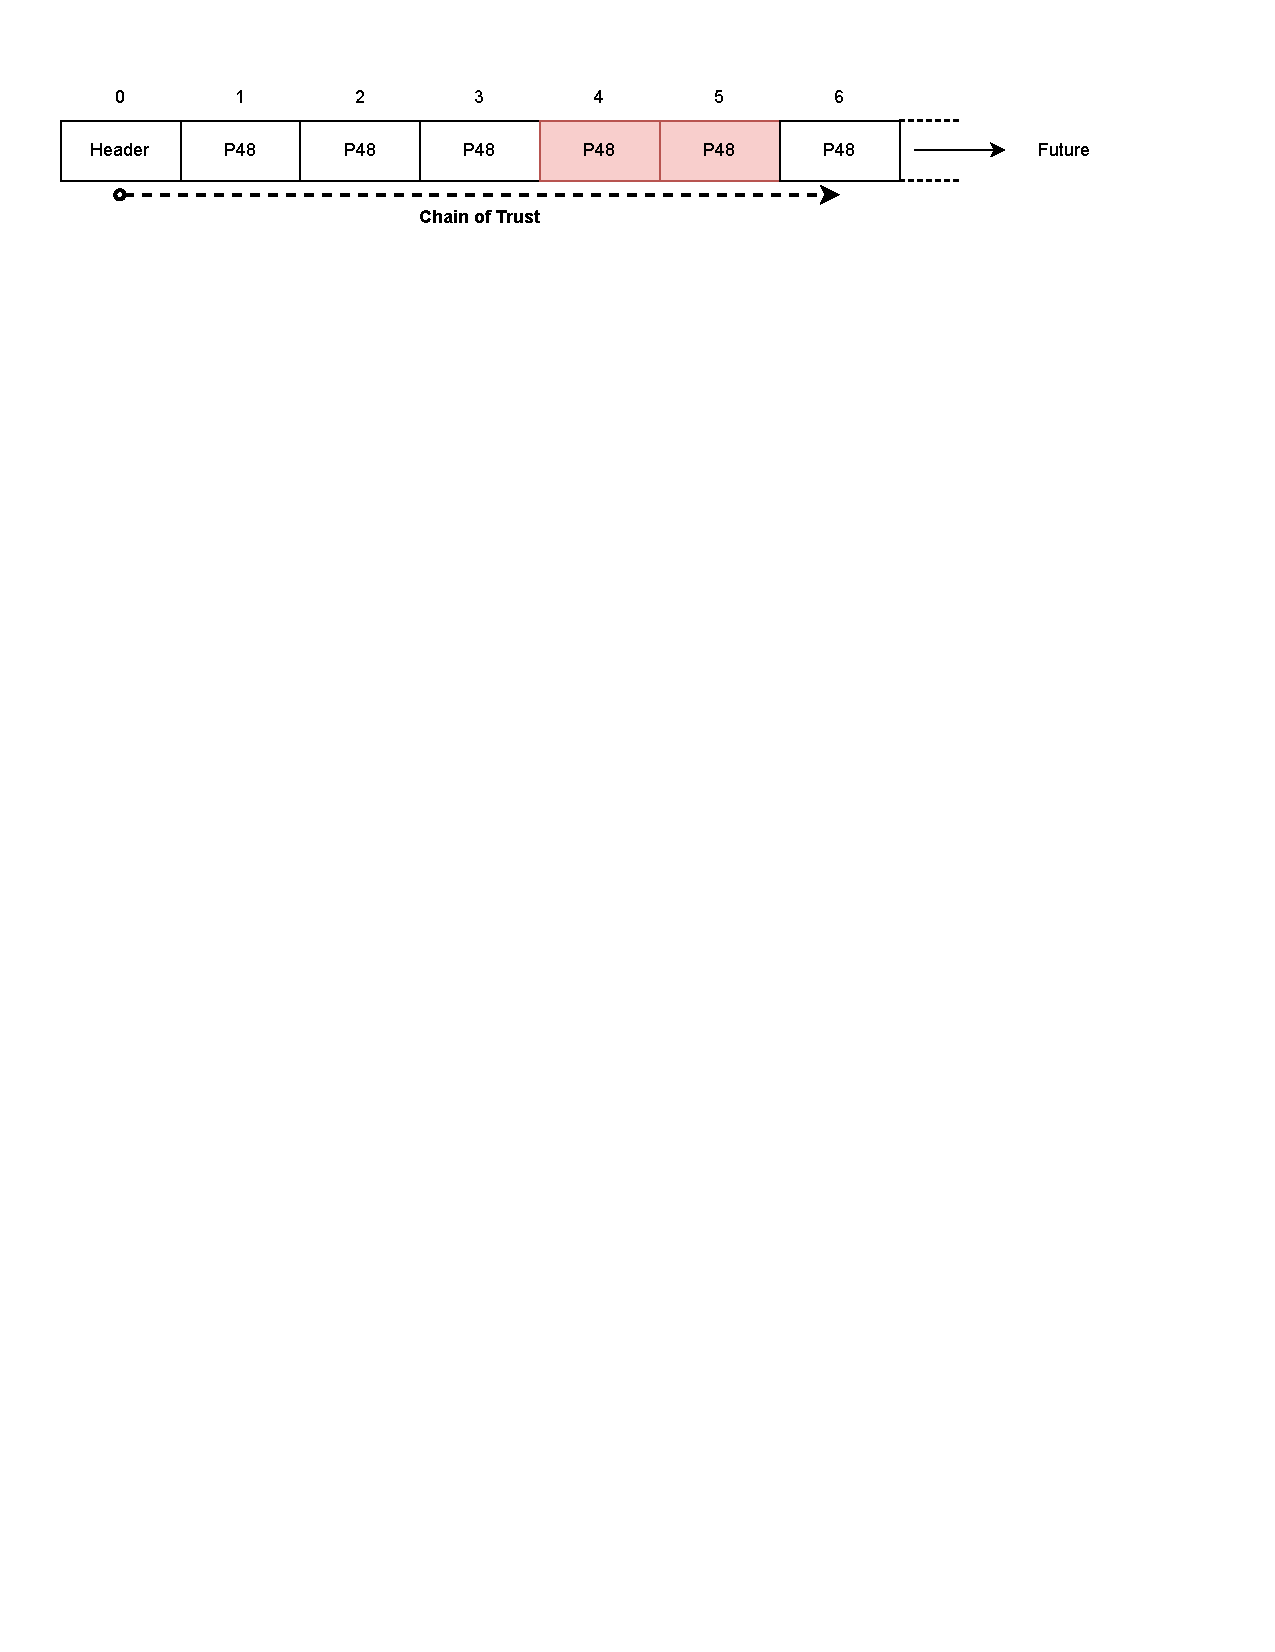
\includegraphics[width=1\textwidth]{images/fork_1.pdf}
        \begin{itemize}
        		\item E.g. Update Feed (Old packets are still of importance)
	\end{itemize}
\end{frame}

\begin{frame}[c]{Simple Fix}
        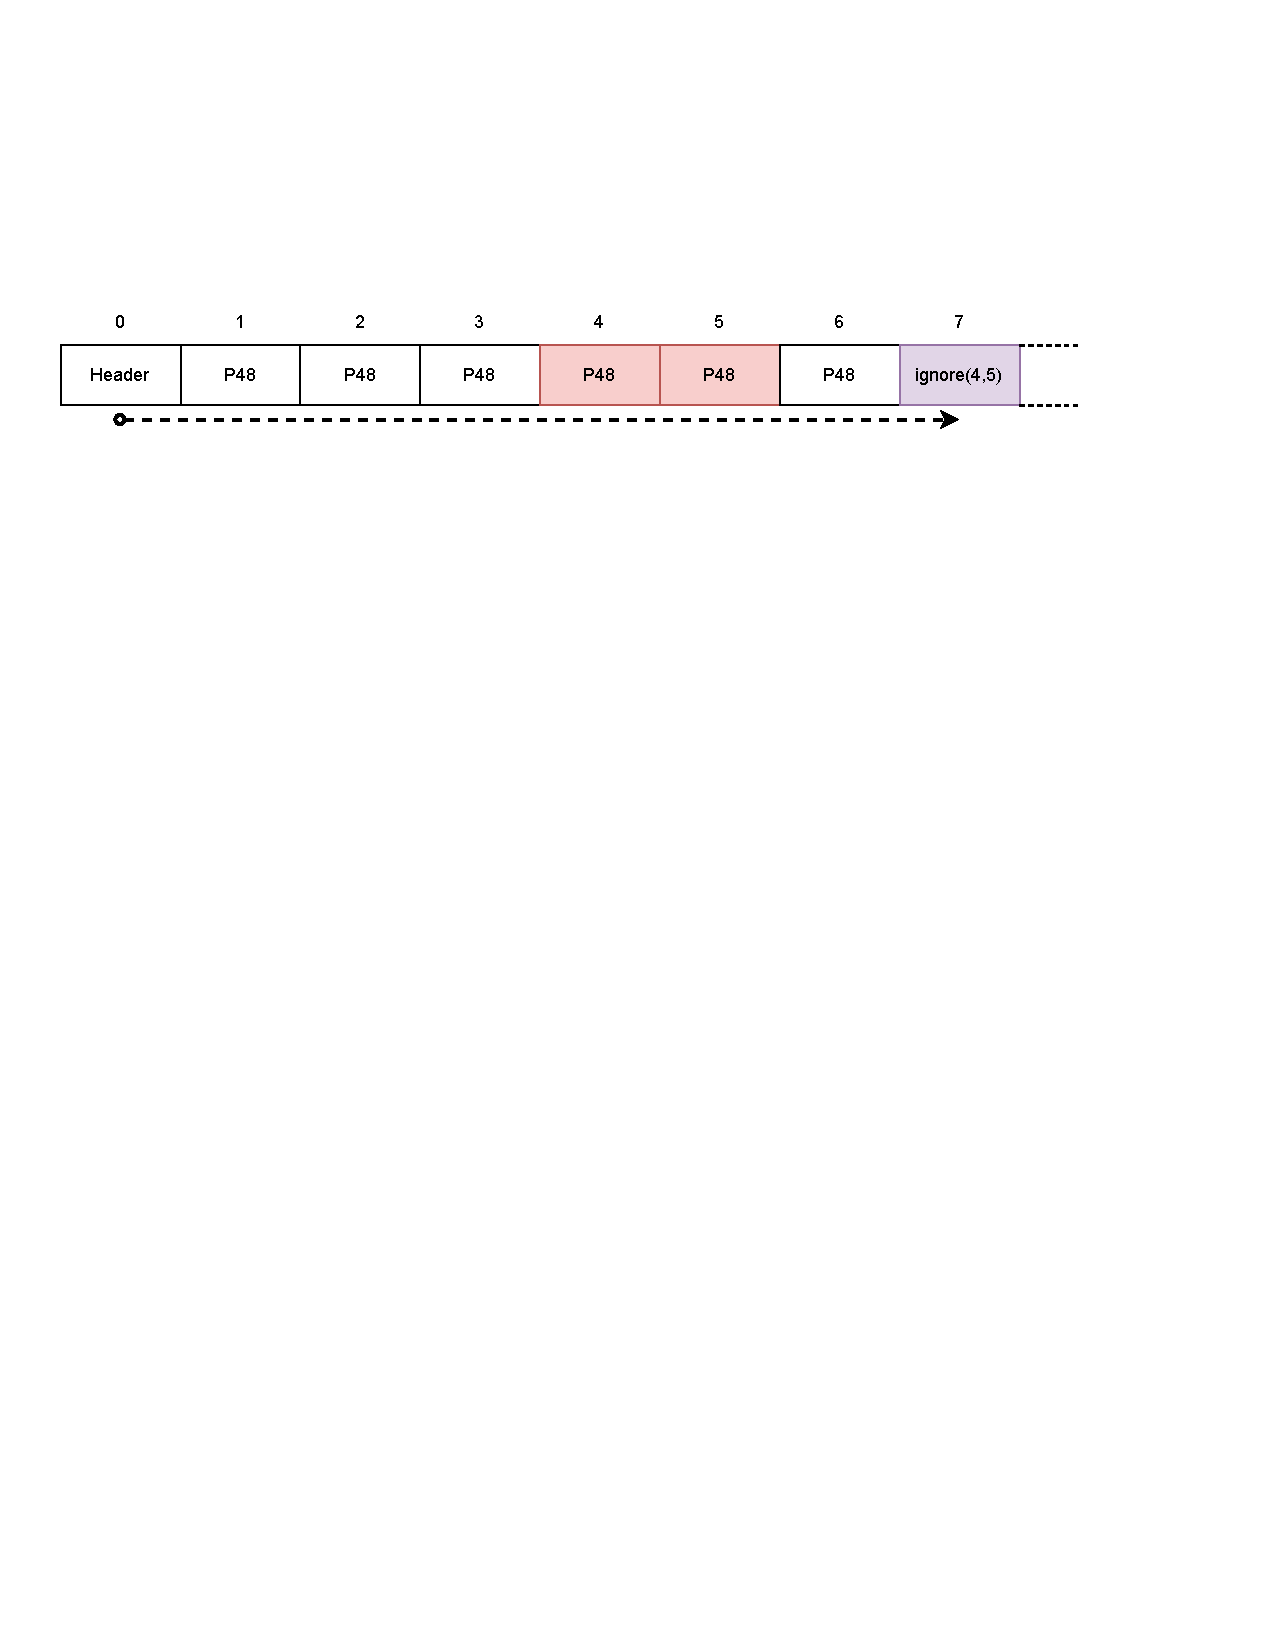
\includegraphics[width=1\textwidth]{images/fork_2.pdf}
        \begin{itemize}
        		\item (+): faulty packets are ignored, simple data structure (feed)
		\item (-): faulty packets still in storage and included in chain of trust
	\end{itemize}
\end{frame}

%\begin{frame}[c]{Limitation: Reverting Packets}
%        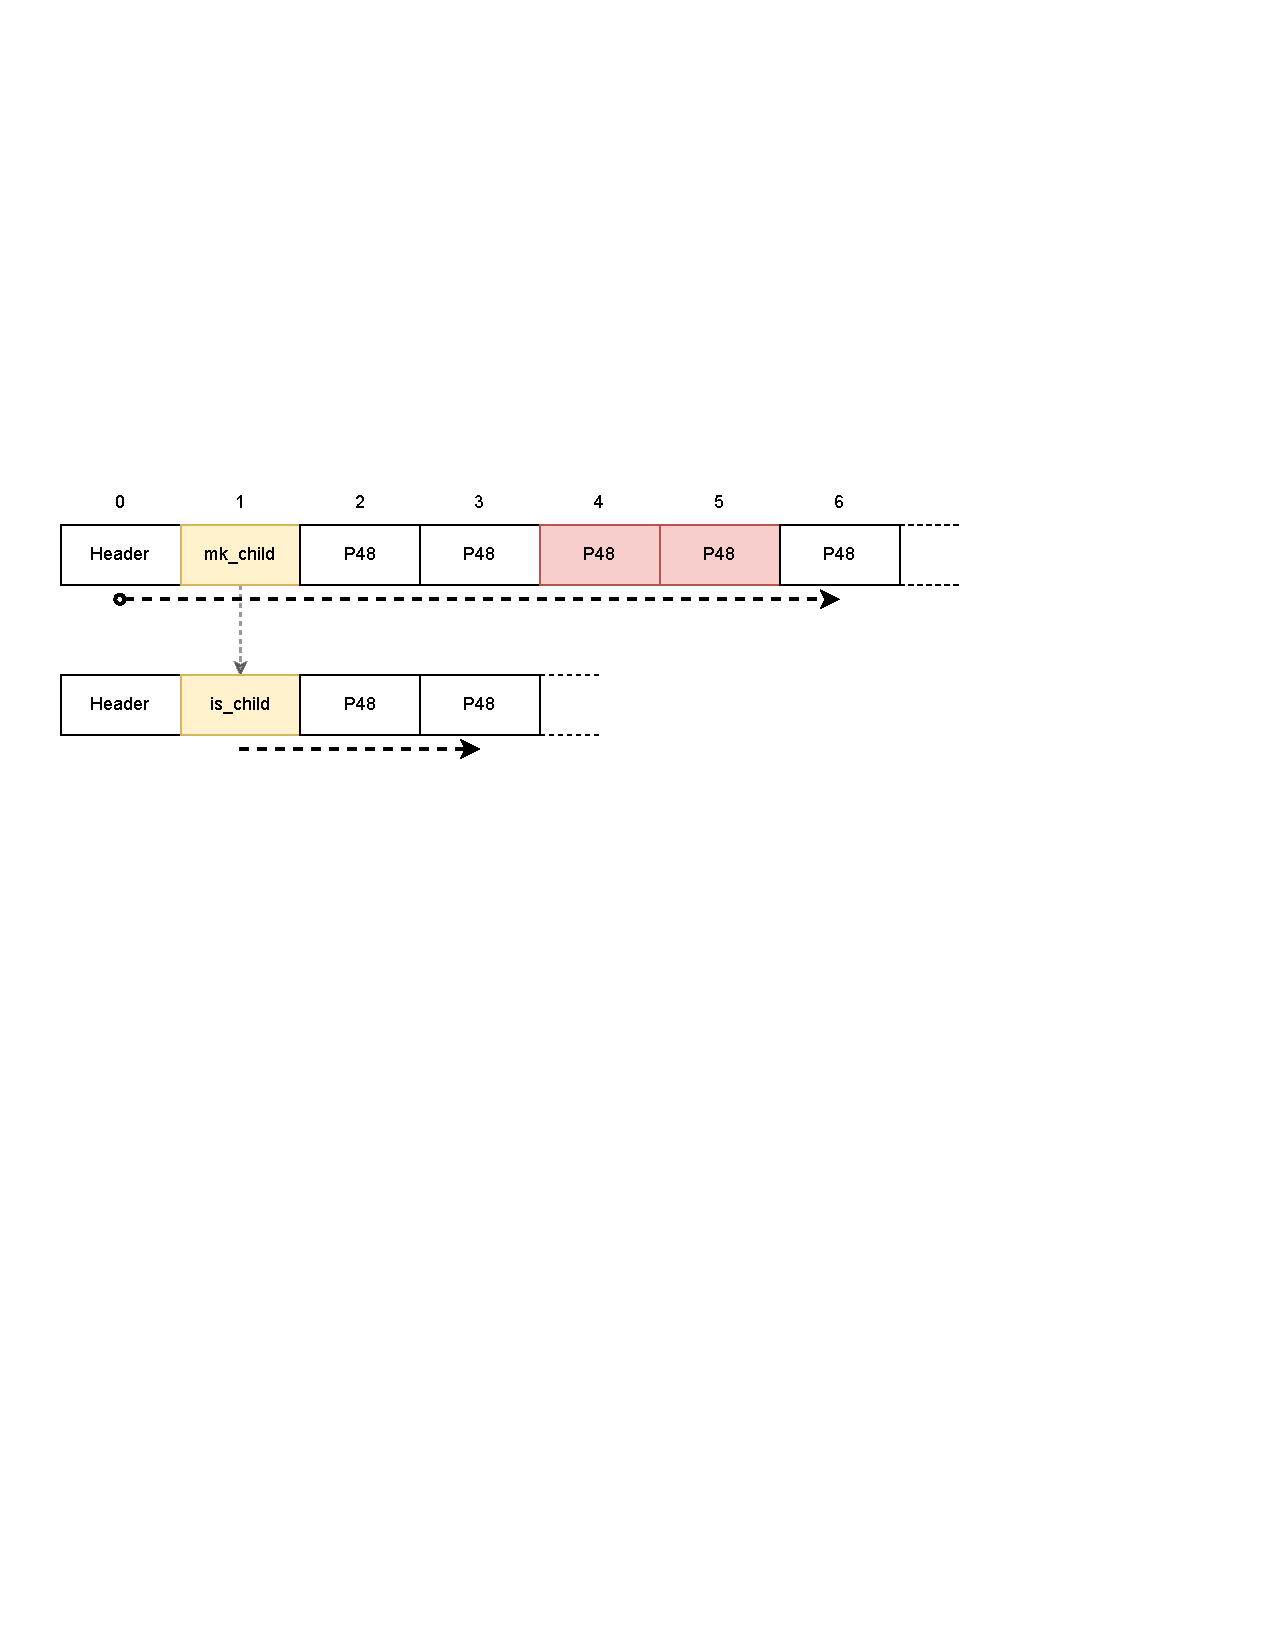
\includegraphics[width=1\textwidth]{images/fork_3.pdf}
%        \begin{itemize}
%        		\item (+): new packets in separate "trust-chain-branch"
%		\item (-): faulty packets still in storage, feed with faulty packets can still potentially grow, unclear where new feed %continues, only one time emergency feed
%	\end{itemize}
%\end{frame}

\begin{frame}[c]{Fork}
        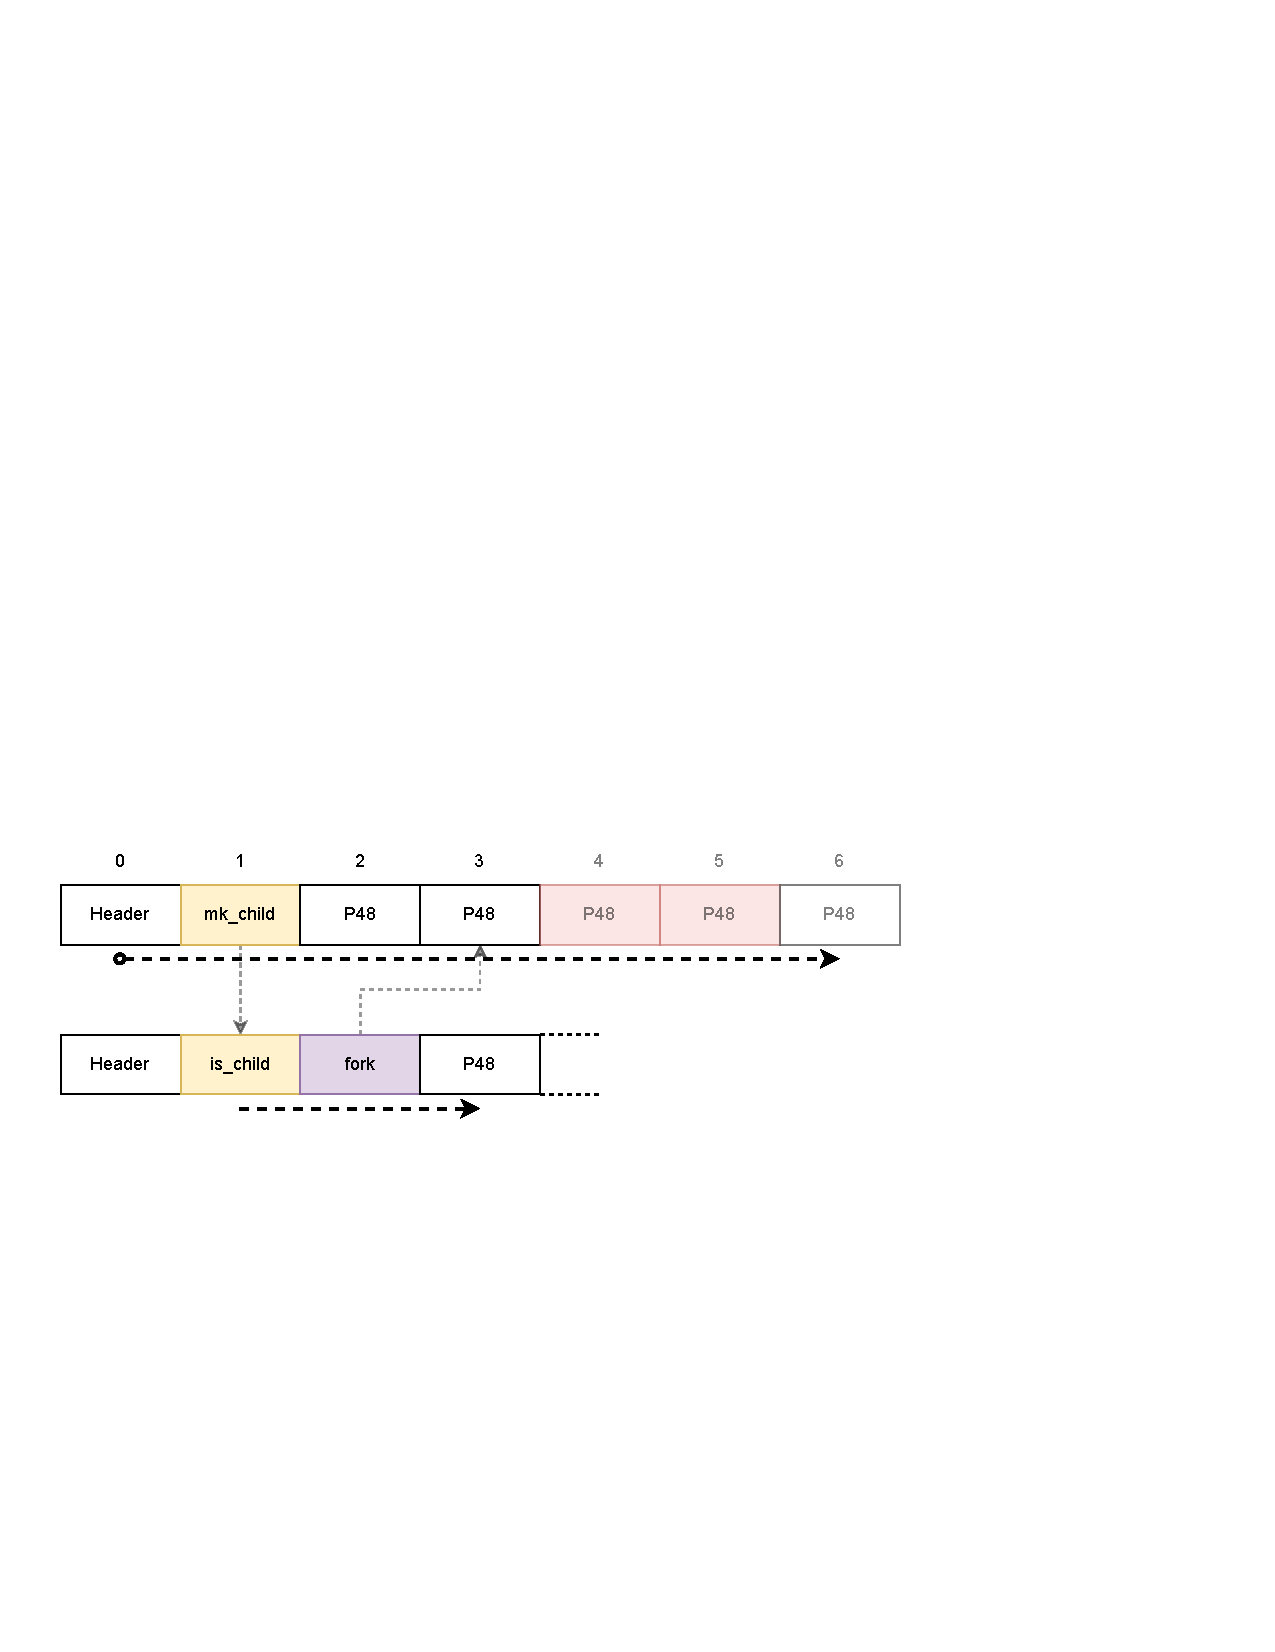
\includegraphics[width=1\textwidth]{images/fork_4.pdf}
        \begin{itemize}
        		\item (+): defined fork position, old feed can stop requesting packets, \\faulty packets can be deleted
		\item (-): only one time emergency feed
	\end{itemize}
\end{frame}

\begin{frame}[c]{Solution: Fork Tree}
        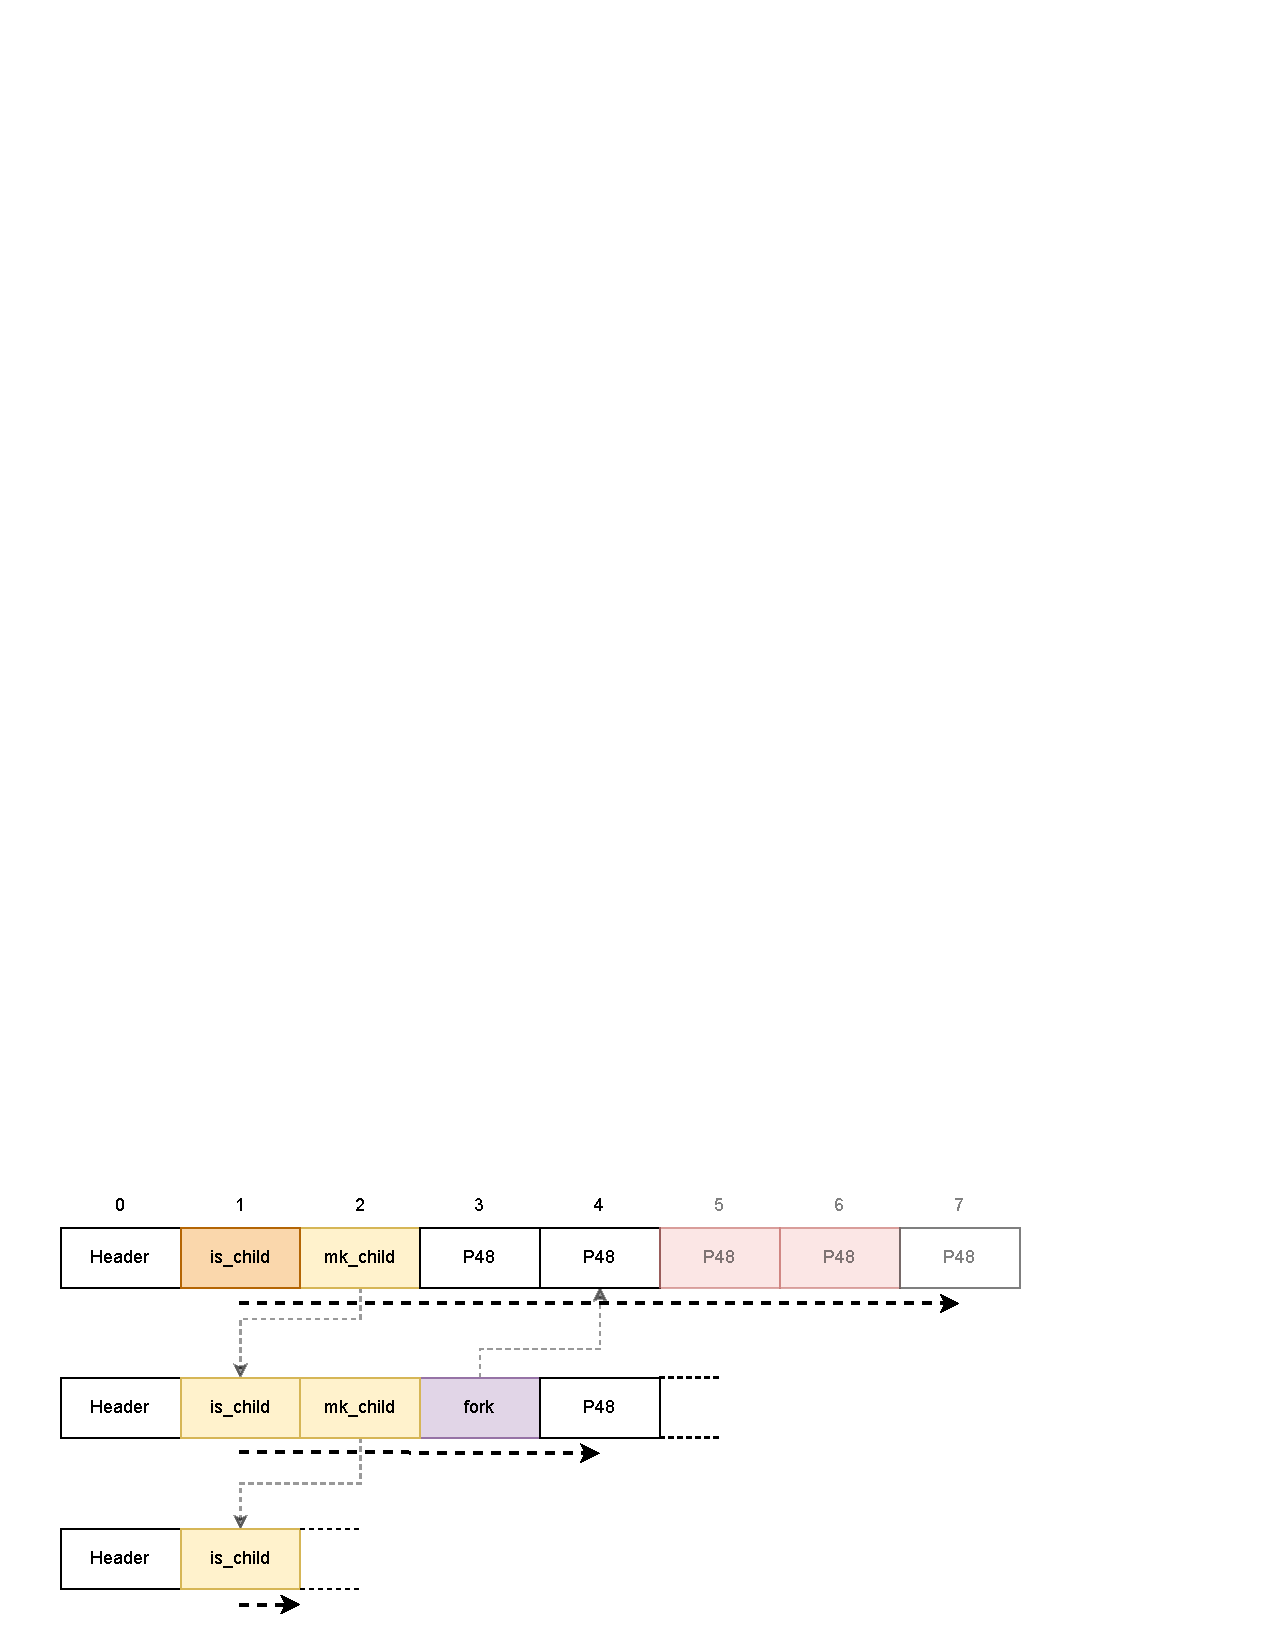
\includegraphics[width=0.8\textwidth]{images/fork_5.pdf}
        \begin{itemize}
        		\item (+): no emergency feed limit
		\item (-): more complex data structure (some storage and requesting overhead compared to single feed)
	\end{itemize}
\end{frame}

\begin{frame}[c]{Limitation: Deleting Old Packets}
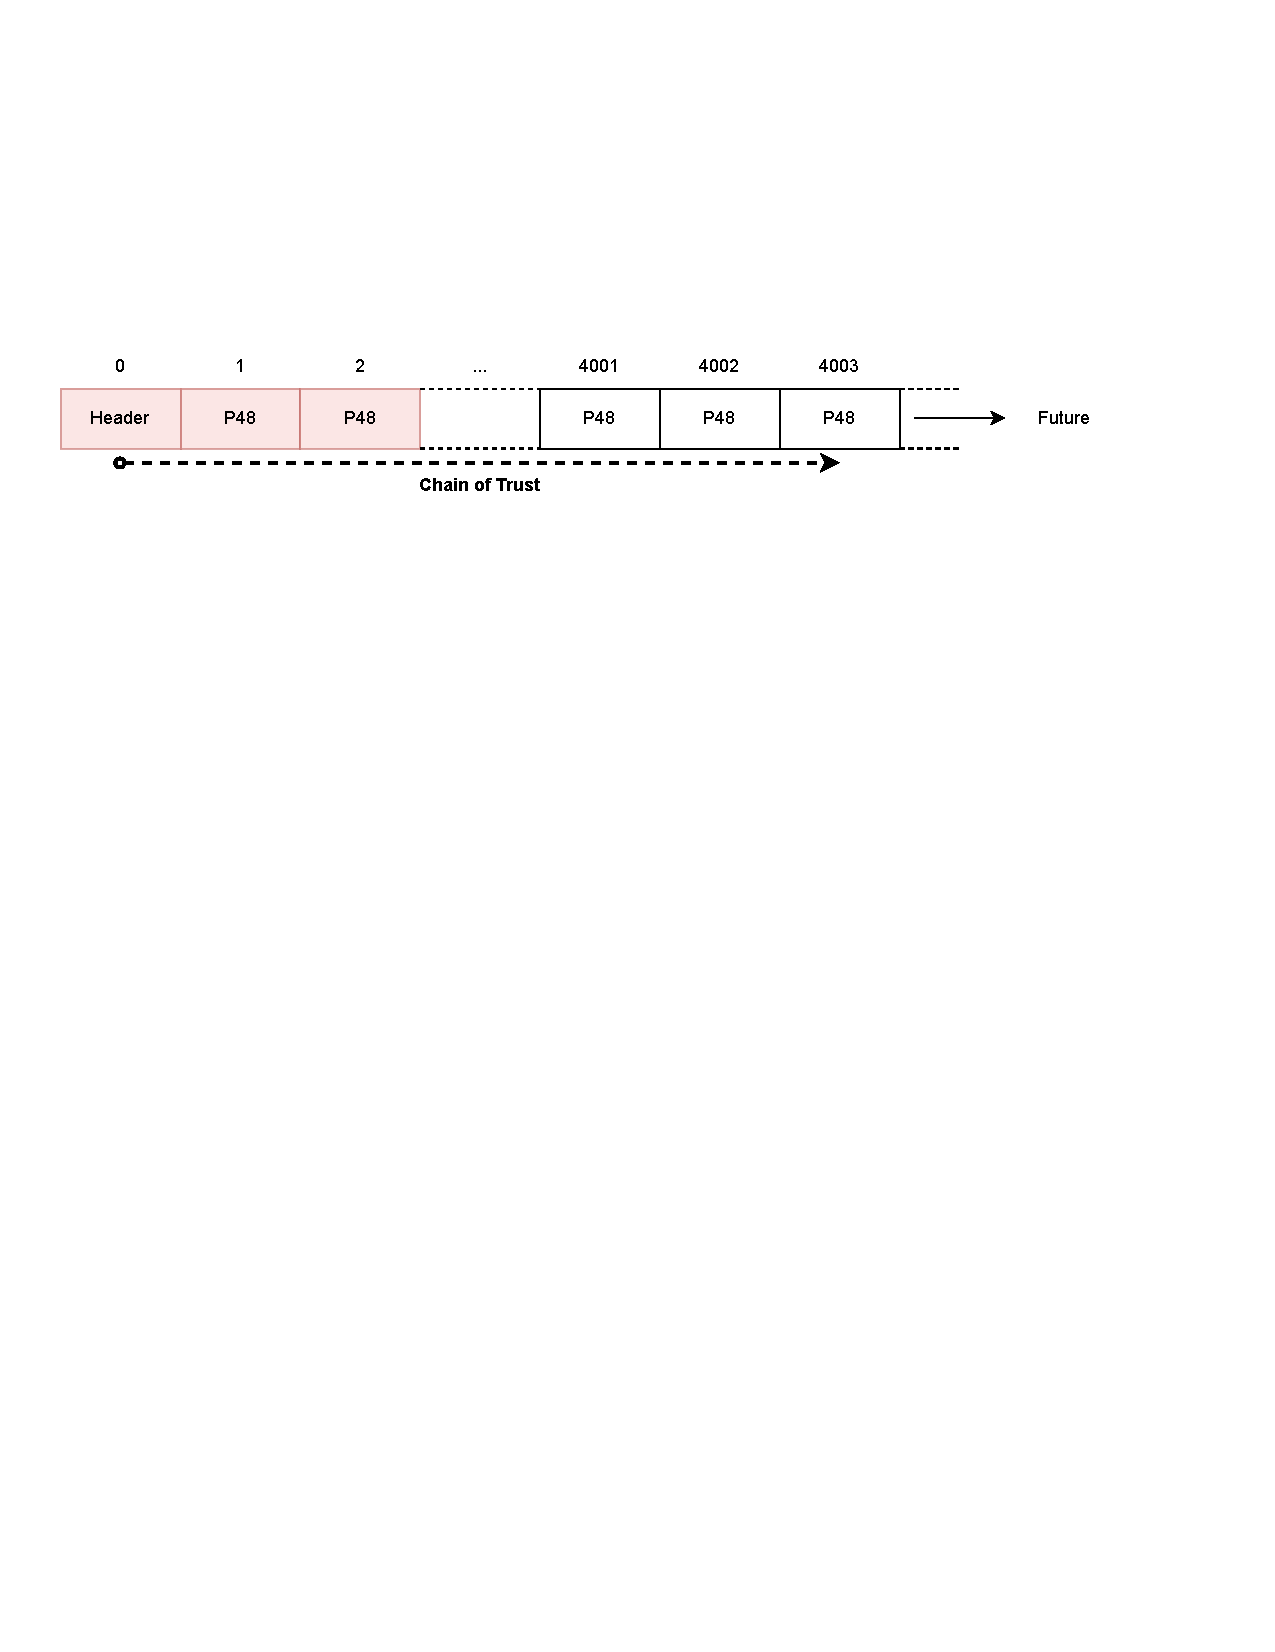
\includegraphics[width=1\textwidth]{images/session_1.pdf}
\begin{itemize}
	\item E.g. Weather Data (Packets not depending on previous packets)
\end{itemize}
\end{frame}

\begin{frame}[c]{Quick Fix}
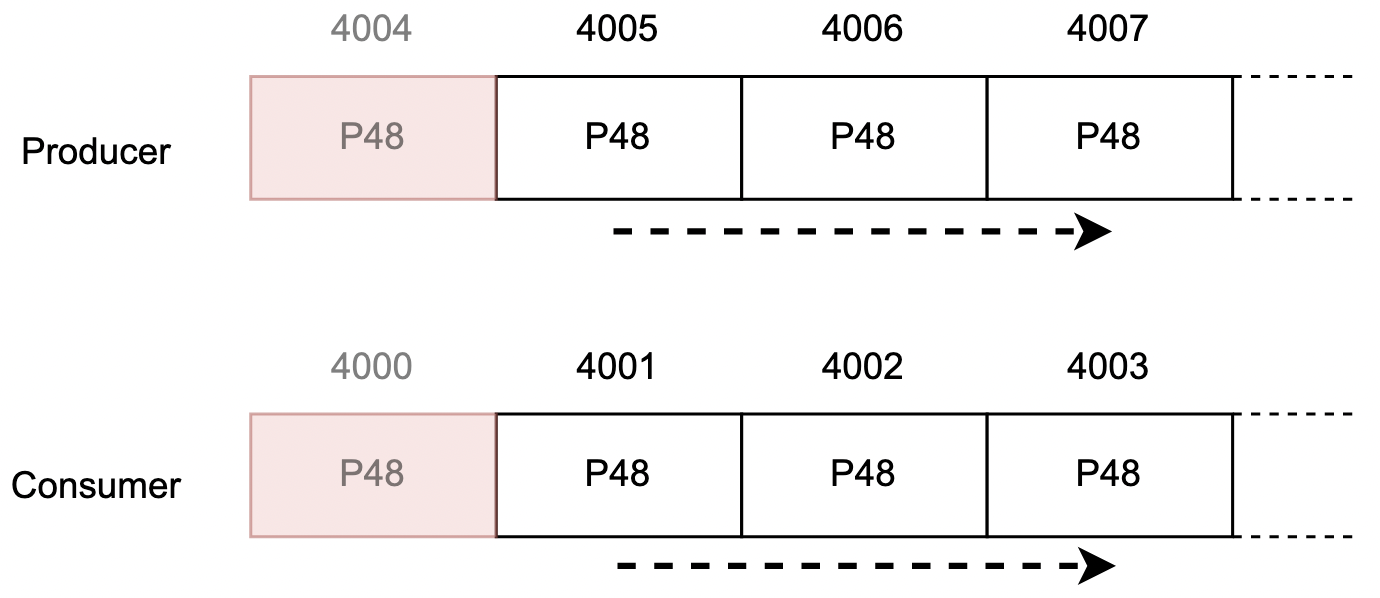
\includegraphics[width=0.5\textwidth]{images/session_2i.png}
\begin{itemize}
	\item (+): Storage problem solved on producer node
	\item (-): Consumer may lose chain of trust
\end{itemize}
\end{frame}

\begin{frame}[c]{Continuation Feeds}
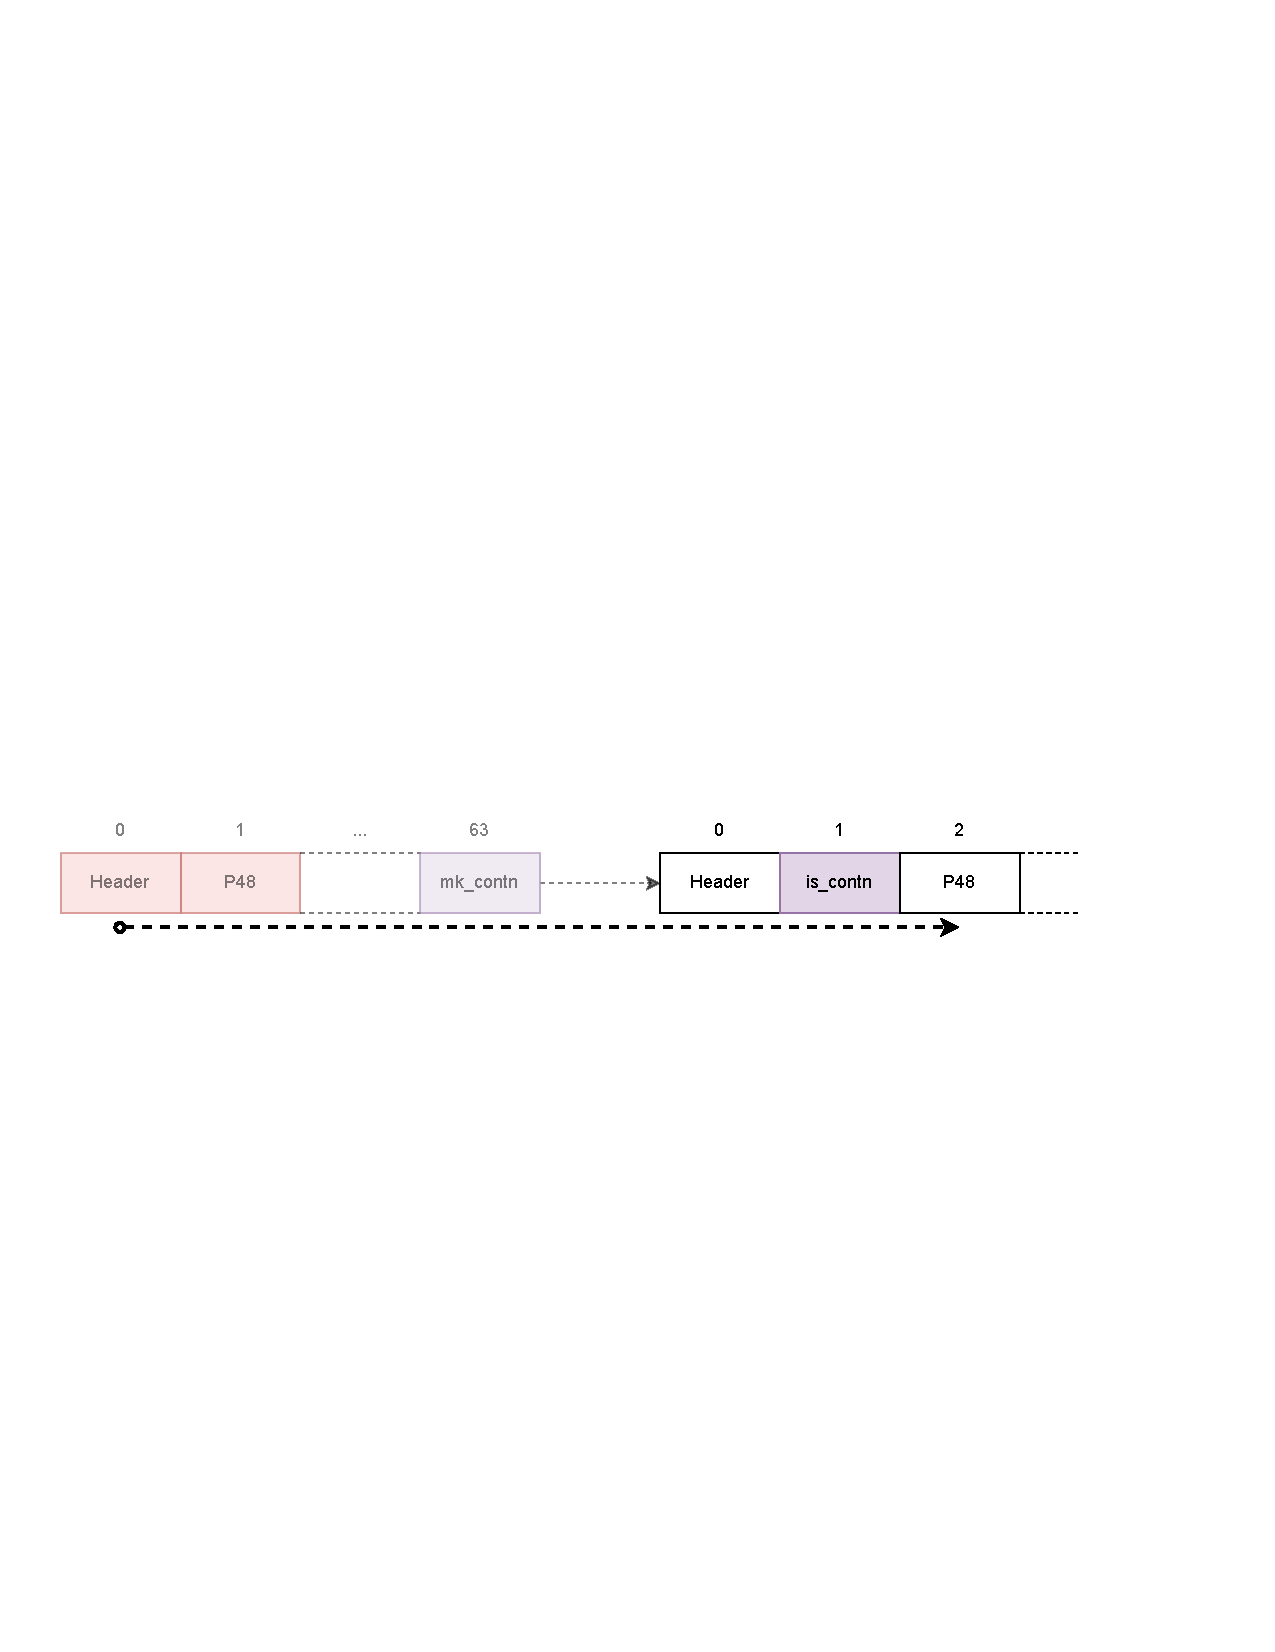
\includegraphics[width=1\textwidth]{images/session_3.pdf}
\begin{itemize}
	\item (+): Storage problem solved on producer node
	\item (-): Consumer may lose chain of trust
\end{itemize}
\end{frame}

\begin{frame}[c]{Deleting Old Feeds}
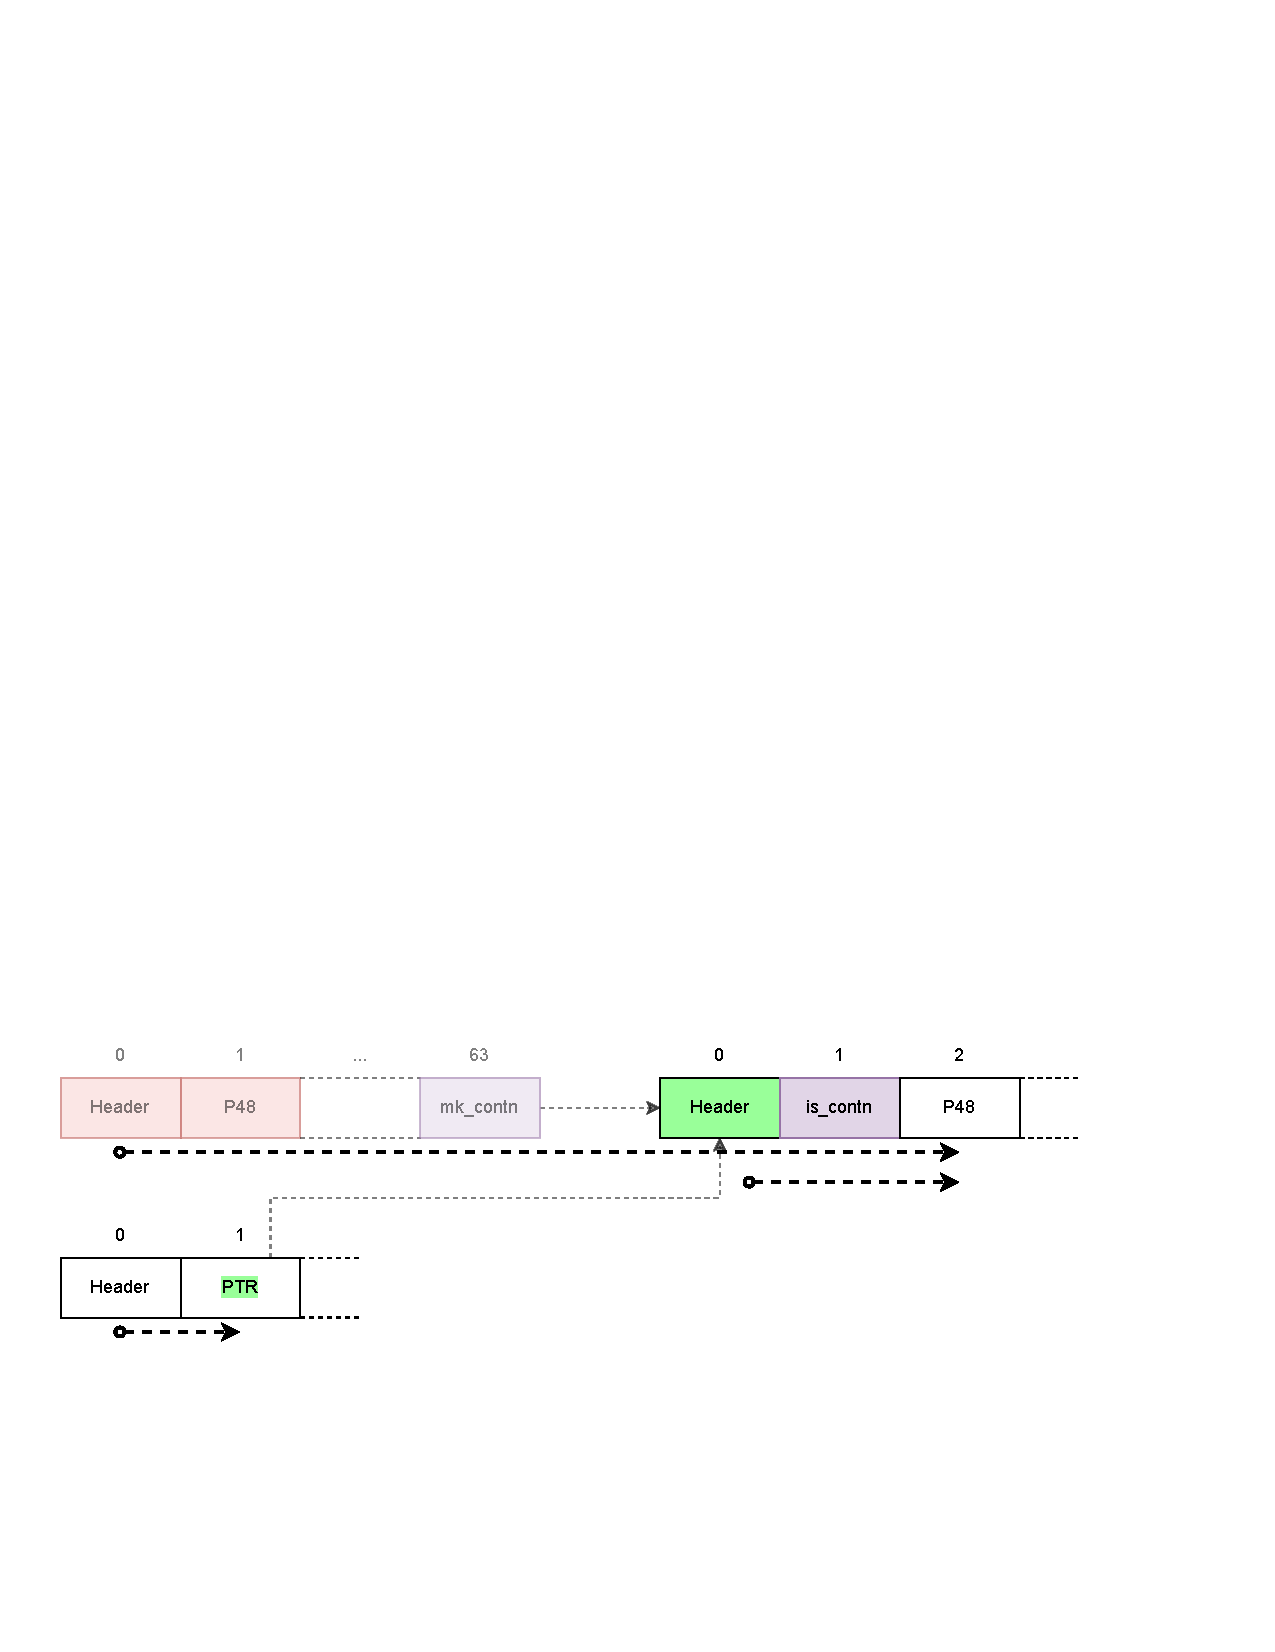
\includegraphics[width=1\textwidth]{images/session_4.pdf}
\begin{itemize}
	\item (+): Old feeds can be deleted, Consumer reaches new feeds
	\item (-): More complex data structure, Pointer Feed can get large
\end{itemize}
\end{frame}

\begin{frame}[c]{Solution: Session-Tree}
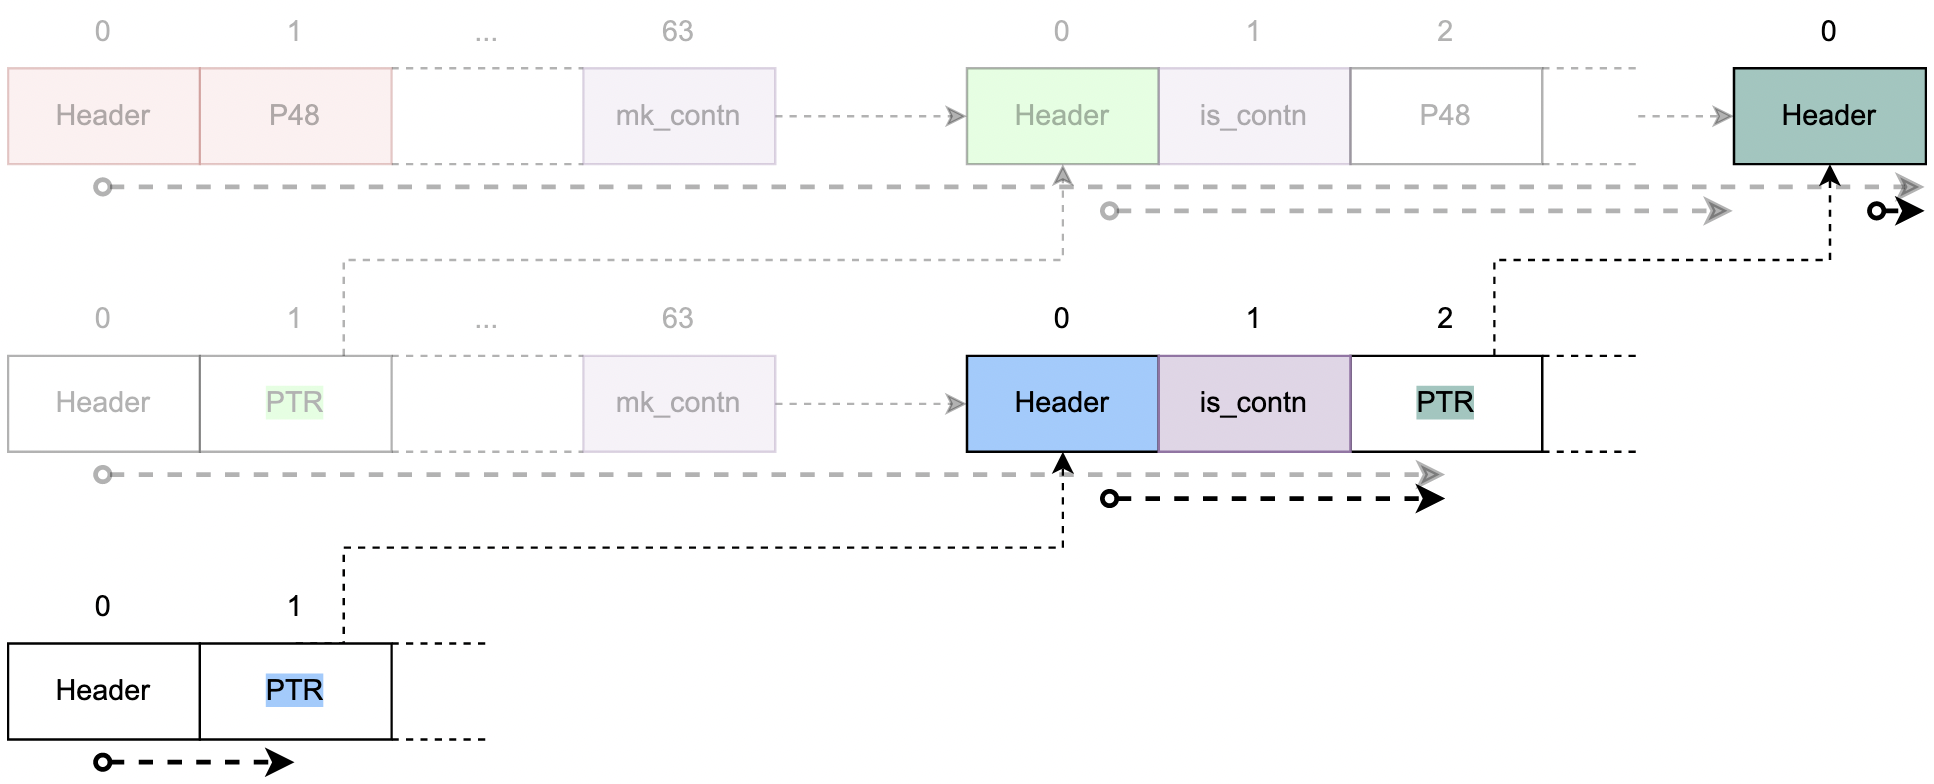
\includegraphics[width=0.9\textwidth]{images/session_5i.png}      
\end{frame}

\begin{frame}[c]{Solution: Session-Tree}
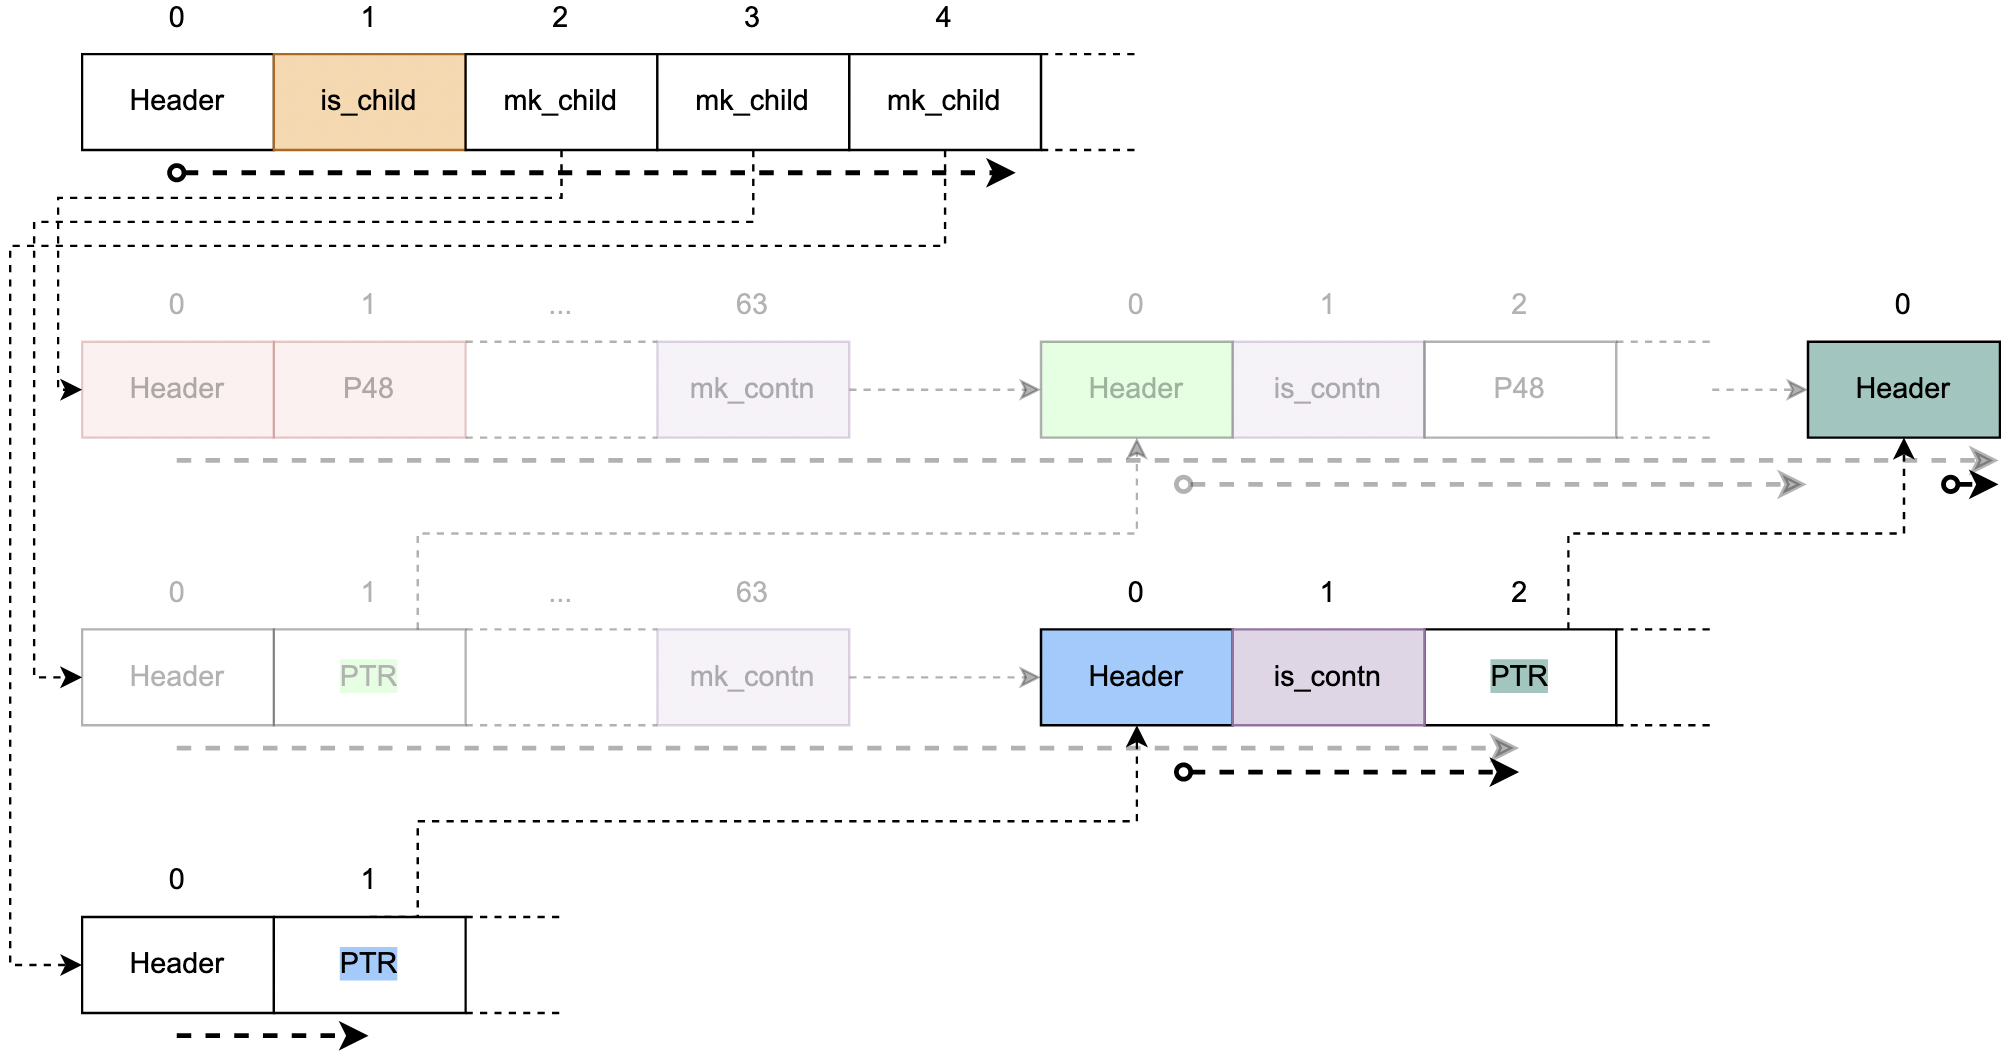
\includegraphics[width=0.9\textwidth]{images/session_6.png}      
\end{frame}

\begin{frame}[c]{Storage and Energy Usage}
\begin{itemize}
	\item Trees have different storage limitation strategies
	\item Energy consumption reduced with efficient packet requesting / handling
\end{itemize}
\end{frame}

% ----------------------------------------------------------------
\section{Demo}

\begin{frame}[c]{Real Life Test}
%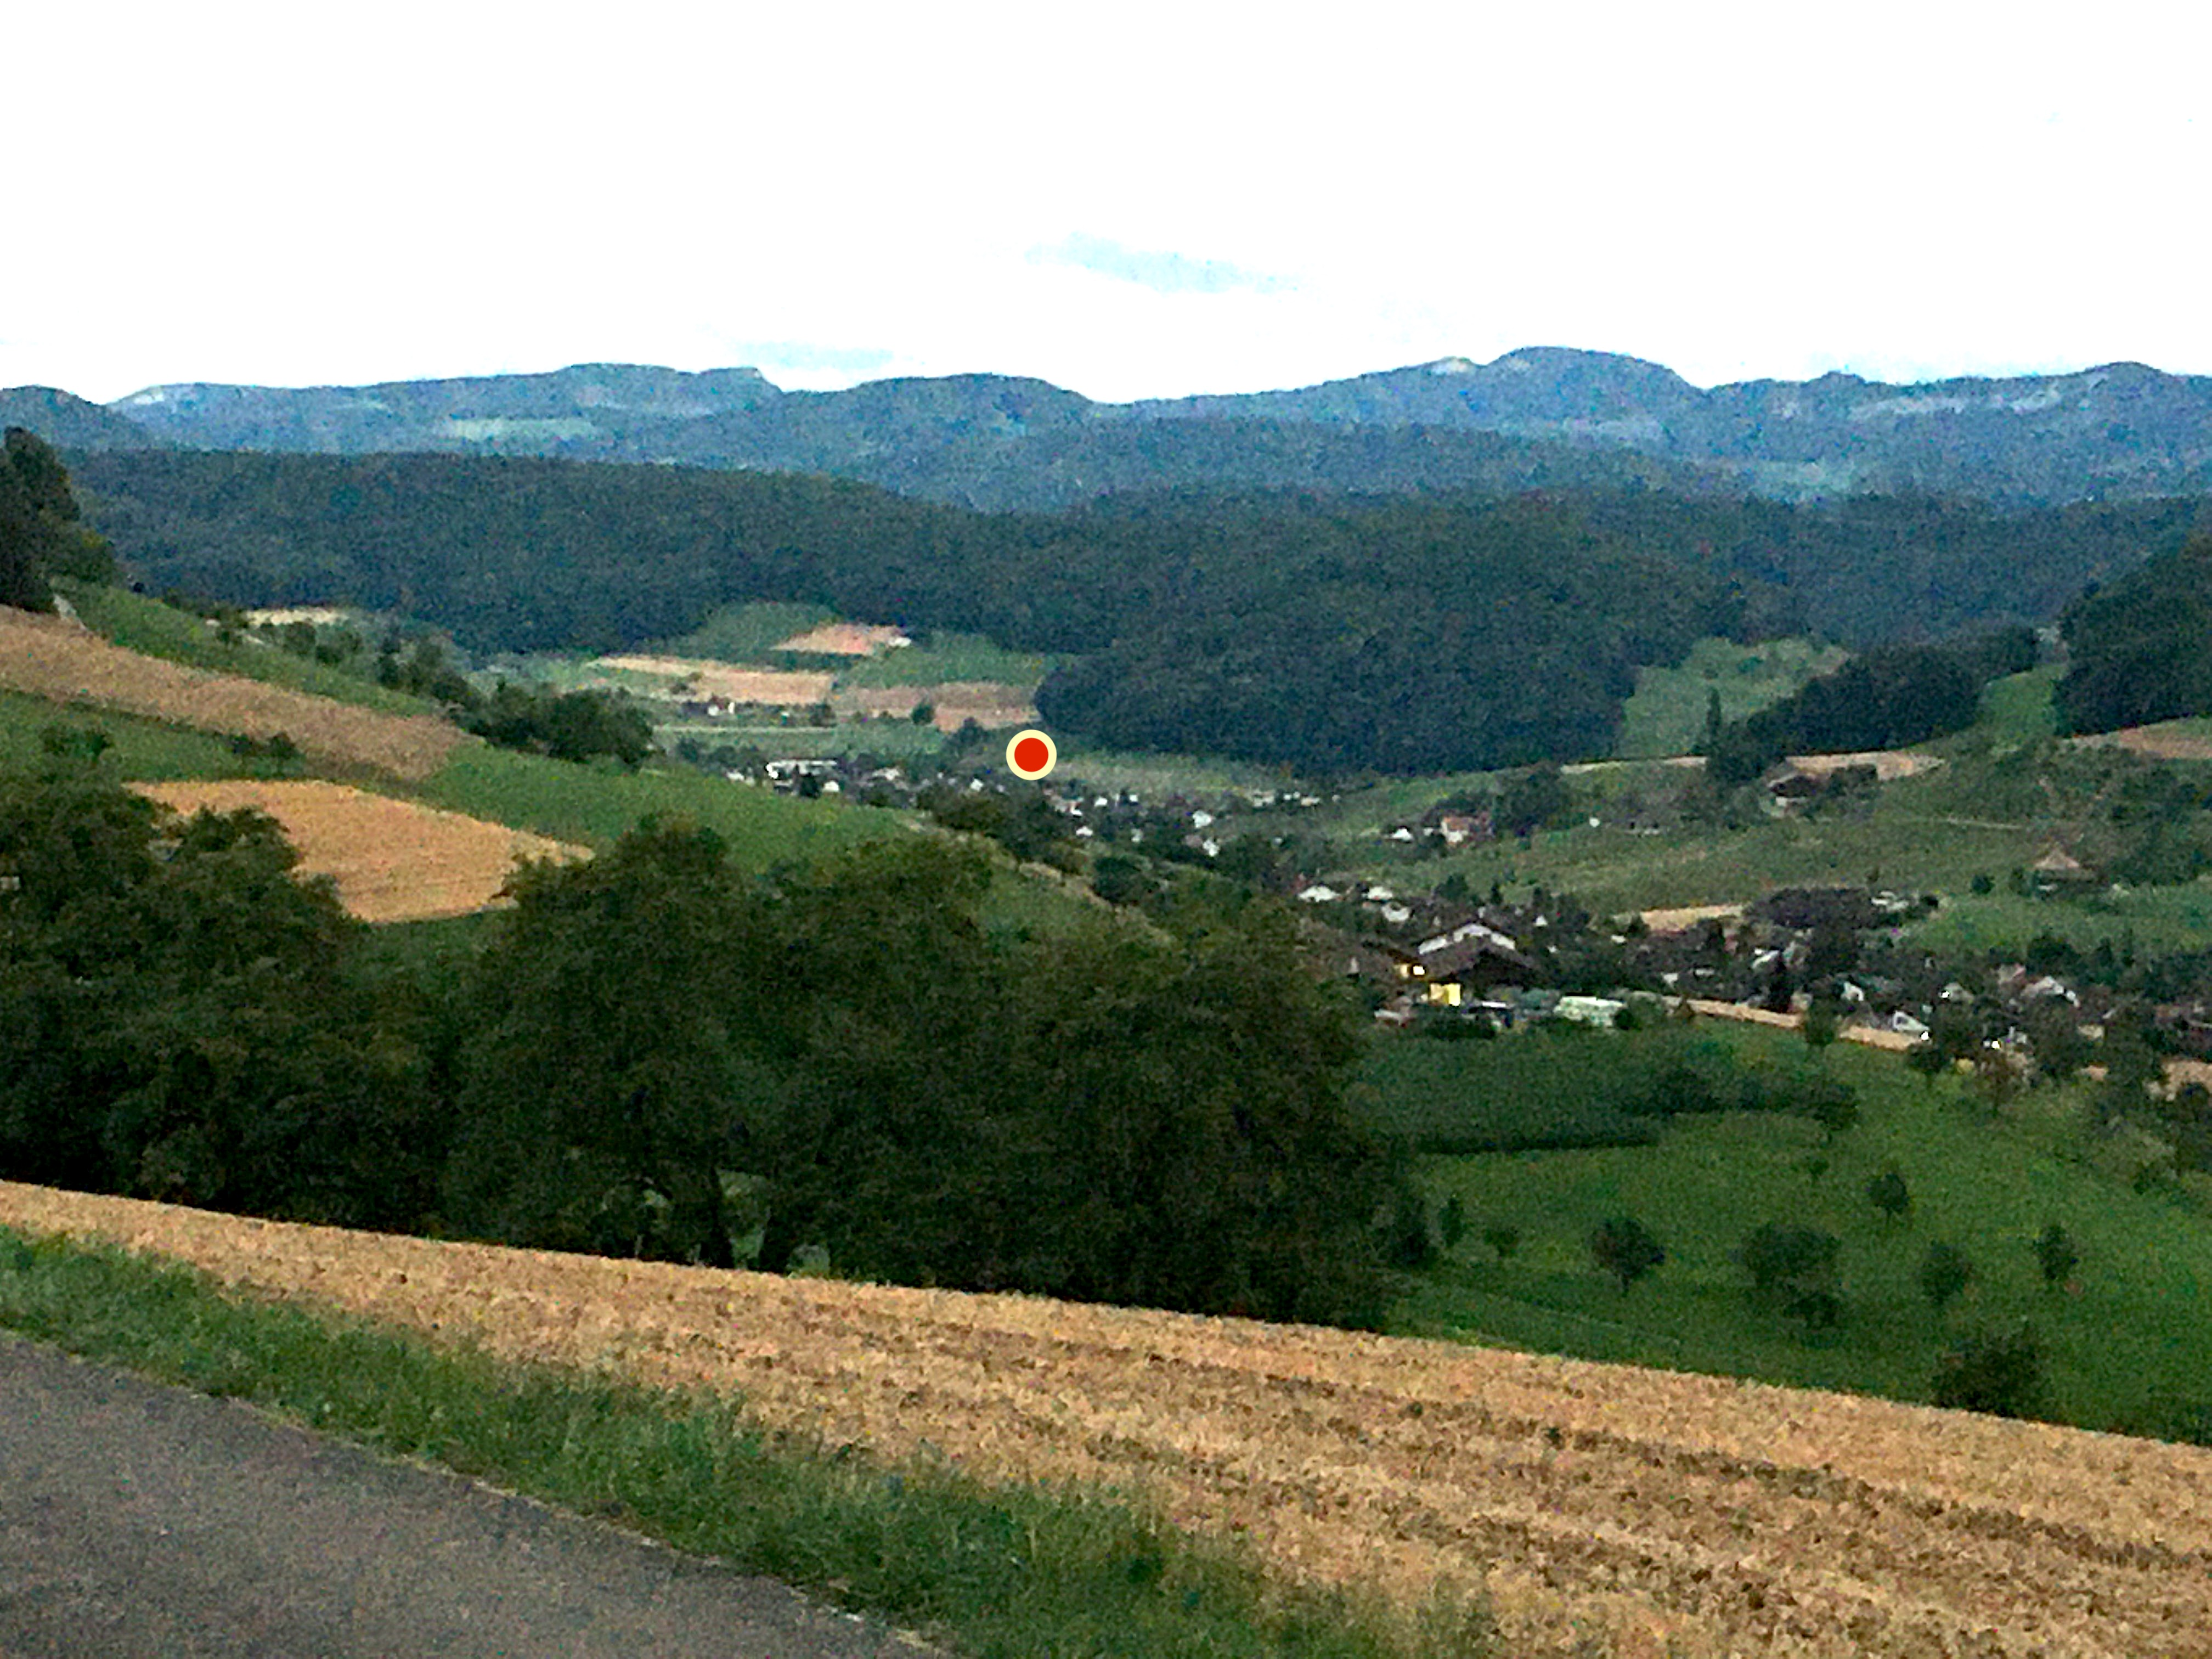
\includegraphics[width=0.5\textwidth]{images/poc_1.JPG}
%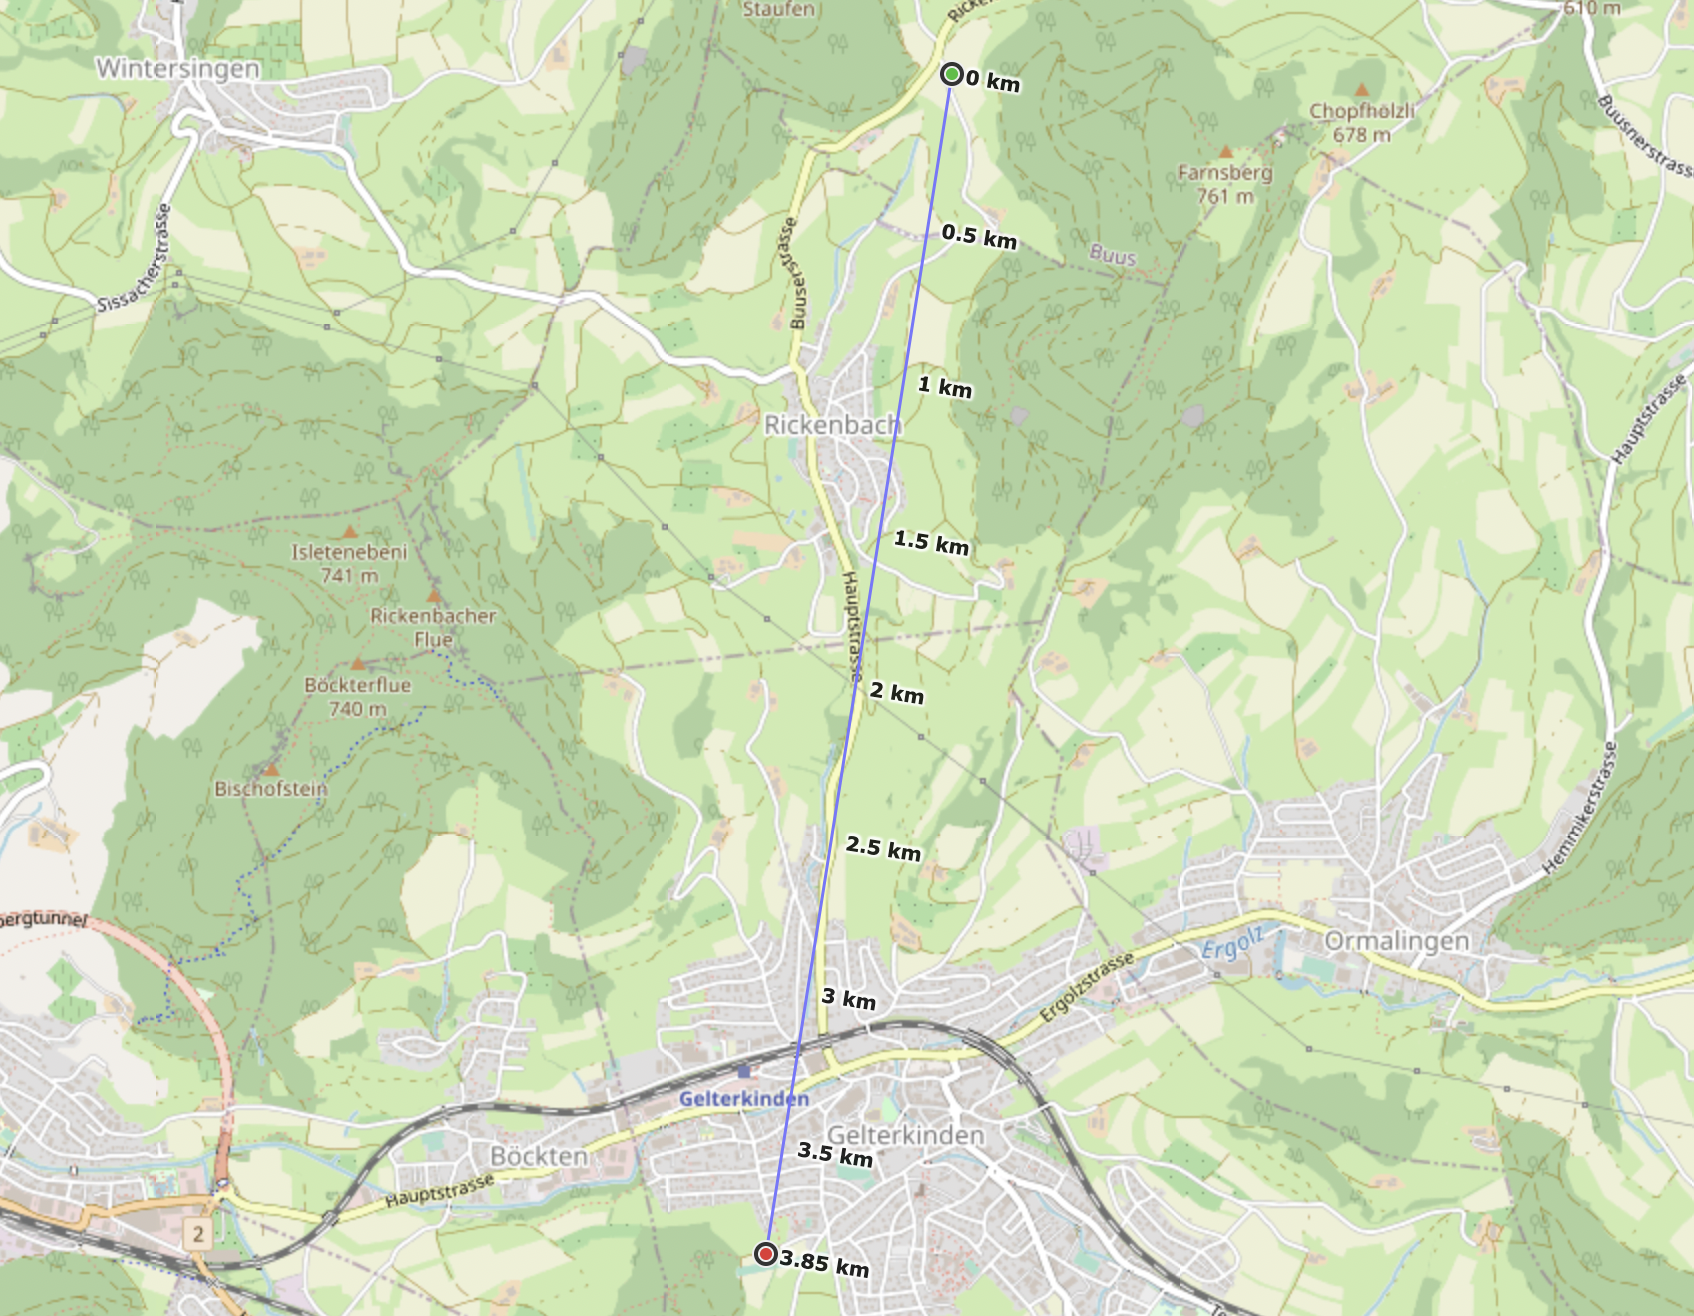
\includegraphics[width=0.5\textwidth]{images/poc_2.png}


\begin{figure}
        \begin{columns}
            \column{.5\linewidth}
            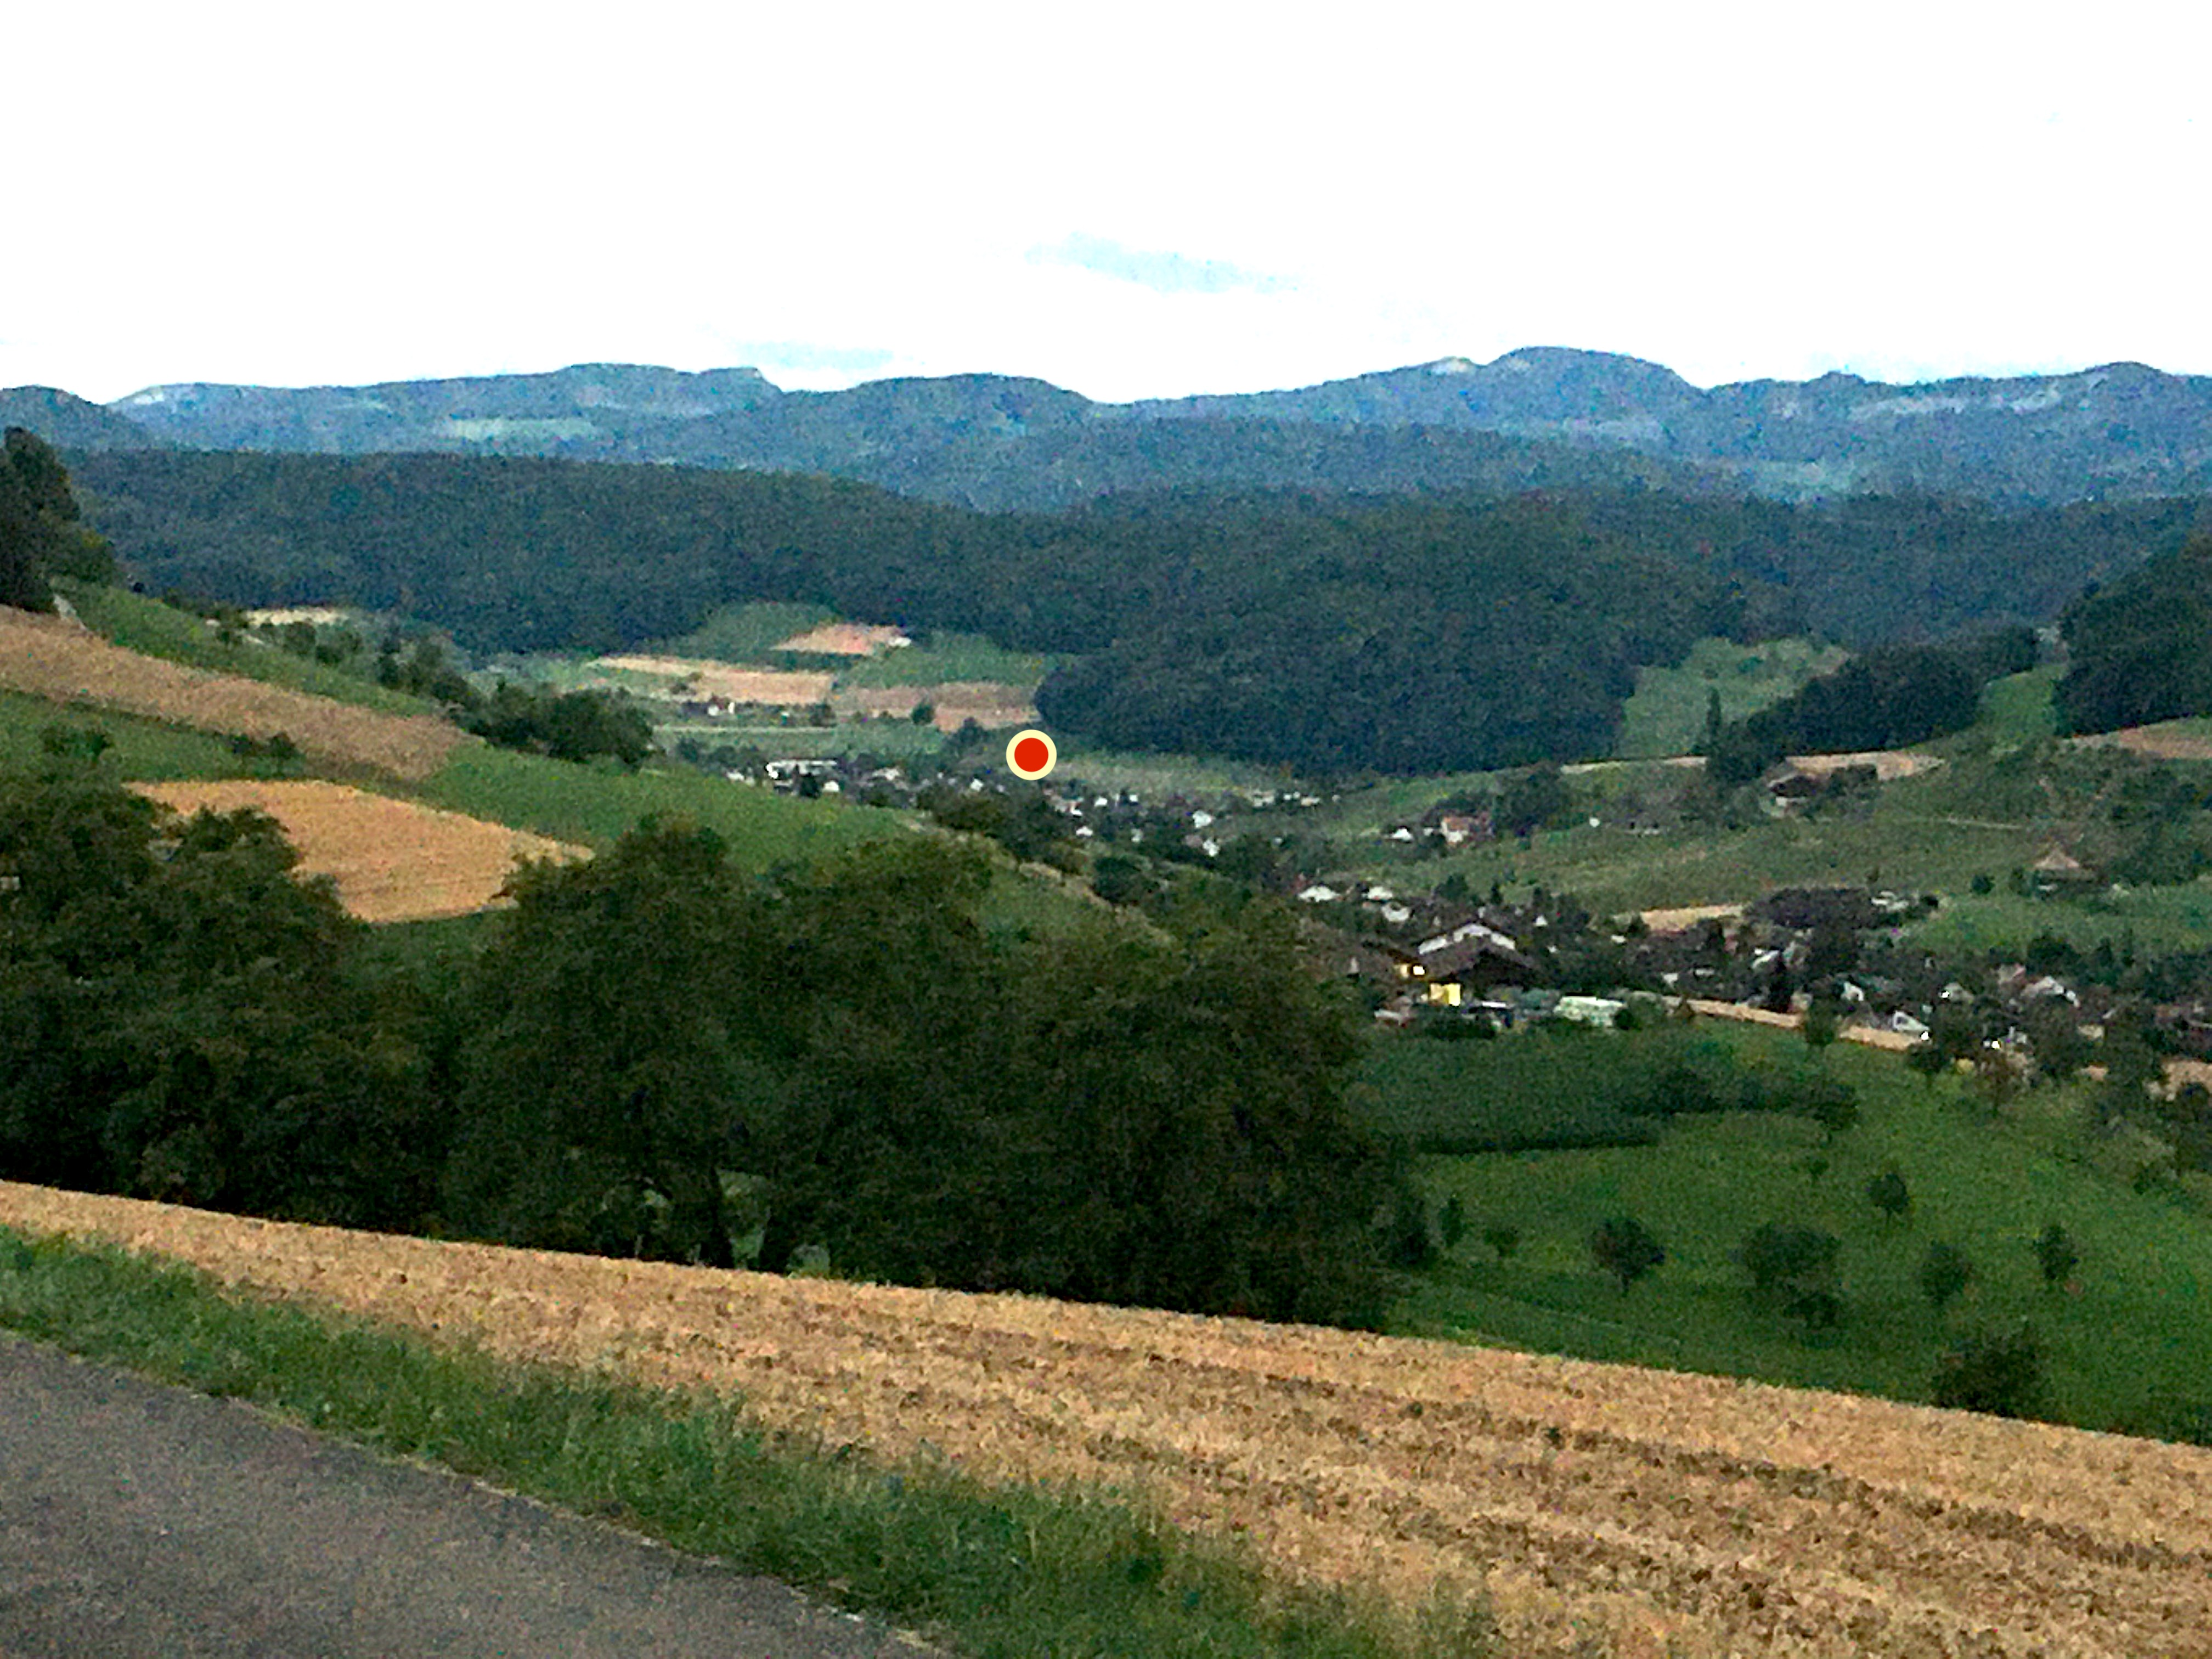
\includegraphics[width=1\textwidth]{images/poc_1.JPG}
            \column{.5\linewidth}
            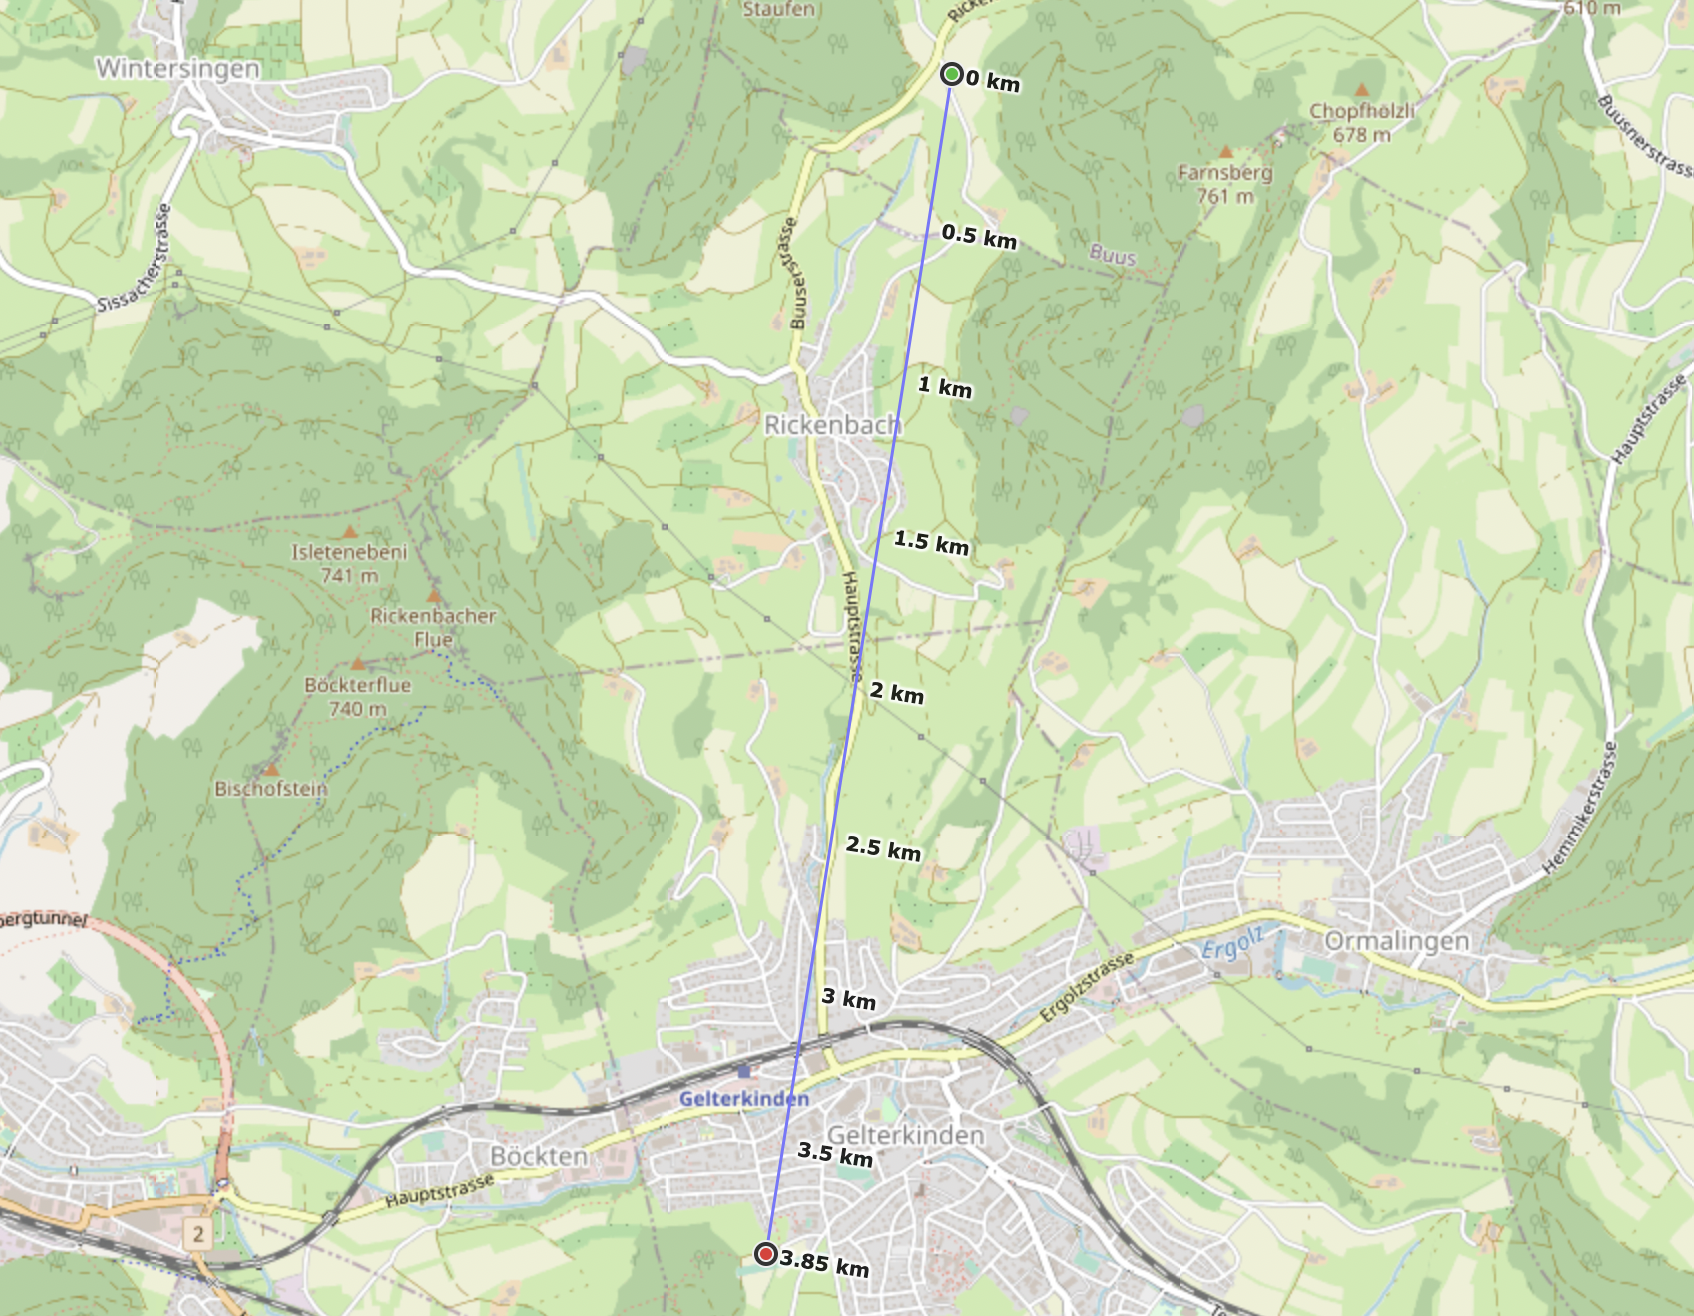
\includegraphics[width=1\textwidth]{images/poc_2.png}
        \end{columns}        
    \end{figure}     
\end{frame}

\begin{frame}[c]{Demo over UDP}
\begin{itemize}
\item Fork-Tree
\item Session-Tree
\end{itemize}

\end{frame}

% ----------------------------------------------------------------
%\section{Future Work}
%\begin{frame}[c]{Future Work}
%\begin{itemize}
%\item Less pointers in Session-Tree
%\item Optimize Packet Requesting (Dynamic Prioritization)
%\end{itemize}
%\end{frame}




\end{document}
